%% P--StwoS.tex
%% Sample file to use for P--S articles prepared in LaTeX
%% For two column P--S articles
%% Version1: Apr 15, 2008
%% Version2: Oct 04, 2013

%% BASIC CLASS FILE
\documentclass{pnastwo}

%% ADDITIO--L OPTIO--L STYLE FILES Font specification

%\usepackage{pnastwoF}
\usepackage{color,capt-of,lipsum}
%\usepackage[square,sort,comma,numbers]{natbib}


%% OPTIO--L MACRO DEFINITIONS
\def\s{\sigma}
\newcommand{\eref}[1]{(\ref{#1})}
\newcommand{\tableref}[1]{Table \ref{#1}}
\newcommand{\figref}[1]{Fig.~\ref{#1}}
\newcommand{\appref}[1]{Appendix \ref{#1}}
\newcommand{\sectionref}[1]{Section \ref{#1}}

\definecolor{Red}{RGB}{255,0,0}
\newcommand{\red}[1]{\textcolor{Red}{#1}}

\definecolor{Green}{RGB}{50,200,50}
\newcommand{\ndg}[1]{\textcolor{Green}{[ndg: #1]}}  

%%%%%%%%%%%%
%% For P--S Only:
\url{www.pnas.org/cgi/doi/10.1073/pnas.0709640104}
\copyrightyear{2015}
\issuedate{Issue Date}
\volume{Volume}
\issuenumber{Issue Number}
%\setcounter{page}{2687} %Set page number here if desired
%%%%%%%%%%%%

\begin{document}

\title{Subjectivity predicts adjective ordering preferences}

\author{Gregory Scontras\affil{1}{Department of Psychology, Stanford University, Stanford, CA 94305},
Judith Degen\affil{1}{},
\and
Noah D.\ Goodman\affil{1}{}}

\contributor{Submitted to Proceedings of the National Academy of Sciences
of the United States of America}

%%%Newly updated.
%%% If significance statement need, then can use the below command otherwise just delete it.
\significancetext{From English to Hungarian to Mokilese, speakers exhibit strong ordering preferences in multi-adjective strings: ``the big blue box'' sounds far more natural than ``the blue big box.'' Rather than a rigid syntax, we show that an adjective's meaning predicts its distance from the modified noun: less subjective adjectives occur closer to nouns they modify. We therefore find evidence of a broadly applicable linguistic universal, adjective ordering preferences, emerging from general properties of cognition. %This case study of adjective ordering preferences provides evidence for broadly applicable linguistic universals emerging from 
%This finding provides a case study in which universal regularities in language derive from universal psychology of word meaning.\ndg{edit that last sentence.. want a succinct statement of why people should care about adj order.}
}

\maketitle

\begin{article}
\begin{abstract}
{The relative order of adjectives in multi-adjective strings is stable not only among speakers within a language, but among speakers across languages. Why is ``the big blue box'' so much better than ``the blue big box''?
We advance the hypothesis that adjective meaning, specifically the subjectivity of the properties that the adjectives name, determines ordering preferences. To test this hypothesis, we establish reliable empirical measures of the preferences themselves and of adjective subjectivity. We then demonstrate that subjectivity is a strong predictor of adjective ordering preferences.}
\end{abstract}

\keywords{language | ordering preferences | subjectivity | faultless disagreement}

%\abbreviations{SAM, self-assembled monolayer; OTS, octadecyltrichlorosilane}

\dropcap{R}egularities in the behavior of speakers and speech communities provide a window onto the psychology of language. Here we take up one such regularity: adjective ordering. Speakers and listeners exhibit strong preferences when two or more adjectives are used to modify a noun, as in ``the big blue box'' or ``the good smooth purple plastic chair.'' Deviate from the preferred order, and the construction becomes marked. Something feels particularly unwieldy about ``the blue big box,'' even more so with ``the plastic good purple smooth chair.'' 
Why do most strings of adjectives have tightly-constrained order?
%for any string of adjectives, chances are their order is non-arbitrary. 
%The question is why. 
We investigate the role of adjective meaning, specifically the subjectivity of the properties that the adjectives name, in predicting ordering preferences.

Adjective ordering preferences stand as a particularly striking case of regularity in language. More remarkable than their robustness in English is their cross-linguistic systematicity: we continually find the \emph{same} preferences across the world's languages. Hungarian (Uralic), Telugu (Dravidian), Mandarin Chinese, and Dutch are just a handful of languages with pre-nominal adjectives (i.e., languages where adjectives precede nouns) reported to have the same ordering preferences as English \cite{martin1969competence,hetzron1978,dixon1982,sproatshih1991,lapollahuang2004}.  In languages like Selepet (Papuan) and Mokilese (Micronesian) with post-nominal adjectives (i.e., where adjectives follow nouns), these preferences are preserved in the reverse \cite{hetzron1978,dixon1982,sproatshih1991}: the preferences determine the linear distance of an adjective from the noun it modifies.

There have been two general approaches to the investigation of adjective ordering preferences. 
As part of a larger project mapping the syntax and semantics of adjectives (a ``cartographic'' approach, one could say), the linguistics literature advances a universal hierarchy of semantic classes of adjectives. Leading the charge, Dixon set out to uncover language-internal structure by which to organize ordering preferences \cite{dixon1982}. The preferences were assumed to be hard-coded in the grammar; the researcher's job was simply to uncover them. 
Building on the ordering of semantic classes proposed by Dixon, Cinque advanced a fully syntactic account of ordering preferences under which different classes of adjectives populate dedicated syntactic categories which inhabit specialized projections in the syntactic tree \cite{cinque1994}. For example, color adjectives project a Color Phrase, shape adjectives project a Shape Phrase. The Shape Phrase syntactically dominates the Color Phrase; with left-branching structure, hierarchical dominance results in linear precedence. The ultimate source of this rigid structure was immaterial; at issue was a comprehensive and deterministic account of the facts (see \cite{scott2002} for a similar proposal).

Before the grammatical approaches, which map, as it were, the terrain of adjective \emph{structure}, psychological approaches advanced the idea that aspects of adjectives' \emph{meaning} determine their relative order. The trouble lies in deciding precisely which aspects of meaning are relevant. 
Kicking off the enterprise in 1898, Sweet proposed that adjectives which are more closely connected with the noun in meaning occur closer to the noun, and that adjectives with a more specialized meaning occur closer to the noun \cite{sweet1898}. Similarly, Whorf proposed that adjectives describing more ``inherent'' properties occur closer to the noun \cite{whorf1945}. Ziff proposed that adjectives with less context-dependent meaning occur closer to the noun, and that adjectives that felicitously describe a narrower set of nouns occur closer to the noun \cite{ziff1960}. The proposals and others like them circle around similar aspects of adjective meaning in their account of ordering preferences; unfortunately, operationalizing metrics like meaning distance, specificity, inherence, and context-dependence is not a trivial task (but see the attempt in \cite{martin1969determinants}). 
Lacking clear empirical measures of the relevant aspects of adjective meaning, these psychological accounts gave way to the more descriptive, grammatical ones that settle for innate syntax as the ultimate arbiter. 
%Without clear empirical constructs of the aspects of adjective meaning that were meant to determine ordering preferences, these psychological accounts gave way to the more descriptive, grammatical ones that settle for innate syntax as the ultimate arbiter.  %Moreover, the , for a psychological theory of ordering preferences to get off the ground, we would need a mapping hypothesis between the relevant aspects of meaning and the cognitive processes that attend to them.

We revisit the idea that ordering preferences emerge from aspects of adjective meaning, attempting to provide more thorough empirical grounding to these notions;
from the grammatical approach we adopt the strategy of using semantic classes of adjectives to structure our investigation and smooth our data. 
Distilling the psychological proposals that precede us into a single feature, we advance the hypothesis that it is the \emph{subjectivity} of the property named that determines ordering preferences \cite{hetzron1978,quirketal1985,hill2012}.
Less subjective adjectives are reliably more useful at communicating the speaker's intended message; the chance of miscommunication decreases with decreasing subjectivity. 
Perhaps for this reason, less subjective adjectives occur closer to the substantive head of the nominal projection, that is, to the modified noun.  
While subjectivity can be assessed directly (by asking participants), we show it can more reliably be measured as the extent to which two people can disagree about a description without one necessarily being wrong. 
 %informative in that it is less likely that there would be disagreement about judgments; there is little question about what the speaker meant to communicate. 
 In ``the big blue box,'' judgments about bigness are likely less consistent than judgments about blueness; ``blue'' is less subjective than ``big,'' and so it occurs closer to the noun ``box.''

To test the hypothesis that adjective subjectivity predicts ordering preferences, we created and validated empirical measures of the ordering preferences themselves and of an adjective's subjectivity. With reliable estimates of both, we then evaluated the predictive power of subjectivity in adjective ordering preferences.

\section{Ordering preferences}

We began by measuring preferences in adjective ordering. We selected a sample of 26 relatively frequent adjectives from seven different semantic classes discussed in the grammatical literature (size, quality, age, texture, shape, color, material). We then elicited naturalness judgments on adjective-adjective-noun object descriptions, permuting the relative order of the adjectives. Participants (n=45) indicated which ordering of an object description sounded more ``natural'' (e.g., ``the big red apple'' vs.\ ``the red big apple;'' see \emph{Materials and Methods} for details).

For each adjective, we computed its mean naturalness score by averaging ratings of configurations in which it appeared in first position, farthest from the noun. Fig.\ \ref{results} (\emph{naturalness}) plots these mean naturalness scores by adjective class; greater values signal that a class's adjectives are preferred in first position, while lower value indicate that a class's adjectives are preferred in second position, closer to the noun. This preferred distance measure closely tracks class-level ordering hierarchies reported in the literature (\cite{dixon1982,sproatshih1991}).

To independently validate our behavioral measure of ordering preferences, we conducted a corpus study on the same 26 adjectives and measured their mean distance from the noun in phrases with two adjectives. We extracted 38,418 cases from the Switchboard Corpus and the British National Corpus (see \emph{Materials and Methods} for details). Mean distance from the noun for each adjective class is shown in Fig.~\ref{results} (\emph{corpus}); higher values indicate that adjectives from the specified class tend to appear farther from the modified noun. The corpus measure closely tracks the qualitative pattern we measured in our naturalness experiment; quantitatively, the two measures are highly correlated ($r^{2}=0.83$, 95\% CI [0.63, 0.90]), in spite of the fact that the corpus measure includes cases from a superset of the nouns tested in our naturalness experiment. Our naturalness ratings thus operationalize both immediate ordering preferences and speakers' preferences in natural usage.


\section{Subjectivity}

%\ndg{i think we should start with subjectivity judgements, then introduce faultless disagreement as a possibly more robust measure. need to say in the end why we take FD as the key measure --- is it more reliable (eg split-half corr)?}
Next, we measured the subjectivity of the adjectives that were tested in the ordering preferences experiments. We started with a direct measure: participants (n=30) were asked explicitly to rate the ``subjectivity'' of adjective-noun object descriptions (e.g.,  ``old apple;'' see \emph{Materials and Methods} for details).
Fig.\ \ref{results} (\emph{subjectivity}) plots these scores by adjective class; greater values indicate greater subjectivity.

 To establish an ecologically valid and therefore more robust measure, we then operationalized subjectivity as the potential for faultless disagreement between two speakers.\footnote{For a different approach, see Hill \cite{hill2012}, who builds on previous corpus work \cite{wulff2003} to infer adjective subjectivity from surface features of strings.} We had participants (n=40) evaluate whether two speakers could both be right while the speakers produced conflicting object descriptions. For example, an experimental trial would have Mary assert, ``That apple is old,'' then have Bob counter with ``That apple is not old;'' 
participants rated whether both Mary and Bob could be right, or whether one of them must be wrong (see \emph{Materials and Methods} for more details). This measure, the faultless disagreement potential for the adjective at issue, serves as an empirical estimate of adjective subjectivity. 
Fig.\ \ref{results} (\emph{faultless}) plots these scores by adjective class, where a value of 1 signals that a class's adjectives are always amenable to faultless disagreement (i.e., maximally subjective), and a value of 0 indicates that a class's adjectives are never amenable to faultless disagreement (i.e., minimally subjective).
The results of this method were highly correlated with our direct ``subjectivity'' scores ($r^{2} = 0.89$, 95\% CI [0.82, 0.93]), suggesting that the measures they invoke converge in their estimation of adjective subjectivity. %We therefore take our faultless disagreement scores as valid empirical constructs of subjectivity.

\section{Predicting adjective order}

To evaluate the power of subjectivity in predicting adjective ordering preferences, we compared our naturalness ratings to the adjective subjectivity scores.
Faultless disagreement scores account for  88\% of the variance in the naturalness ratings ($r^2$ = 0.88, 95\% CI [0.77, 0.95]; Fig.~\ref{naturalness-faultless-pred}).
The direct ``subjectivity'' scores also perform well, accounting for 81\% of the variance ($r^2$ = 0.81, 95\% CI [0.68, 0.89]).
%At the class level, faultless disagreement scores account for 86\% of the variance ($r^2$ = 0.86, 95\% CI [0.36, 0.99]).
%Given the greater ecological validity and better performance of our faultless disagreement measure, we  
Using either measure, more subjective adjectives are preferred farther from the noun; subjectivity indeed predicts adjective ordering preferences.

One might worry that conducting our analysis at the level of individual adjectives obscures information about the specific adjective-adjective-noun configurations that participants rated in our naturalness experiment.
We therefore computed a subjectivity difference score for each adjective class configuration (i.e., an ordered pairing of two adjective classes, \textsc{class1}-\textsc{class2}) by subtracting the mean faultless disagreement score for \textsc{class2} from the mean faultless disagreement score for \textsc{class1}. Higher difference scores indicate that the adjective class closer to the noun is less subjective than the class farther away. Fig.~\ref{naturalness-faultless} plots mean naturalness ratings for adjective class configurations against these faultless disagreement difference scores; the two measures are highly correlated ($r^2$ = 0.82, 95\% CI [0.71, 0.88]). Performing the same analysis on specific adjective configurations, we find that faultless disagreement difference scores predict 70\% of the variance in the rating data ($r^2$ = 0.70, 95\% CI [0.67, 0.74]), which constitutes 85\% of the theoretical maximum (i.e., variance not due to noise; see \emph{Materials and Methods} for details). The fact that faultless disagreement difference scores account for almost all of the naturalness rating variance strongly supports our hypothesis that less subjective adjectives occur closer to the noun. 

\section{Discussion}

Adjective ordering preferences have received considerable attention throughout the history of generative grammar and cognitive psychology, owing to their remarkable stability within and across languages. Something so robust, the reasoning goes, must evidence a deep principle of the cognitive architecture that shapes language. Yet while descriptions of the phenomenon abound, an explanation has proven elusive. Grammatical theories that posit a rigid syntax of adjective classes offer little more than a codification of the facts, and psychological approaches stumble when it comes to operationalizing the specific aspects of adjective meaning at play. 

In our investigation, we established two empirical constructs: the preferences themselves, which we measured using naturalness ratings and validated with corpus counts; and adjective subjectivity, which we operationalized as potential for faultless disagreement and corroborated with a direct ``subjectivity'' measure. Our findings suggest a clear path forward: an adjective's semantics can indeed predict its distance from the modified noun, such that less subjective adjectives occur linearly closer to nouns they modify. These results suggest that ordering preferences likely emerge from a desire to place less subjective content closer to the substantive head of a nominal construction (i.e., closer to the modified noun). For now we can only speculate about the ultimate source of this desire: less subjective content is reliably more useful at communicating about the world. Subjective content is potentially less useful because it allows for miscommunication that might arise if speakers and listeners arrive at different judgments about a property description. The robust tendency that results consolidates less subjective adjectives around the noun that names the object being described. Whatever its source, the success of subjectivity in predicting adjective ordering preferences evidences a case where language universals, the regularities we observe in adjective ordering, emerge from cognitive universals, the subjectivity of the properties that the adjectives name.

\begin{materials}
\section{Experiment 1: Naturalness ratings}	
We recruited 50 participants through Amazon.com's Mechanical Turk crowd-sourcing service. Participants were paid \$0.30 for their participation.
Participants were asked to indicate which of two descriptions of an object sounded more natural. Each description featured a noun modified by two adjectives, for example ``the red small chair'' or ``the small red chair''. Description pairs contained the same words, with relative adjective order reversed. Descriptions were random combinations of two adjectives and a noun from the list in Table \ref{stim-table}, with the constraint that no description contained adjectives from the same semantic class.
On each trial, participants indicated their choice by adjusting a slider with endpoints labeled with the competing descriptions; an example trial appears in Fig.\ \ref{order-trial}. Participants completed 26 trials. On each trial, we measured the distance of the slider from each endpoint; values ranged between 0 and 1. Only native speakers of English with IP addresses located within the United States were included in the analyses; we analyzed data from 45 participants.

%We analyzed the obtained slider values by interpreting the scale as ranging from 0 to 1. For each scale label, we interpret it as the zero point and compute the distance of the slider from it as its order preference value.



\section{Experiment 2: Corpus counts} 
We used TGrep2 \cite{rohde2005} and the TGrep2 Database Tools \cite{degenjaeger-tdt} to extract all ``A A N"  NPs that contained one of the 26 adjectives in Table \ref{stim-table} from the Penn Treebank subset of the Switchboard corpus of telephone dialogues \cite{godfrey1992}, as well as from the spoken and the written portions of the British National Corpus (BNC, see http://www.natcorp.ox.ac.uk/). For these cases, we computed the distance of each occurrence of our 26 target adjectives from the modified noun, yielding results for a total of 38,418 adjective tokens.  For each adjective, mean distance from the noun was computed (where the position directly preceding the noun was coded as 0, and the position preceding that was coded as 1). The same procedure was used to compute mean distance by adjective class.
%To determine which differences between adjective classes are meaningful differences, we conducted Bonferroni-corrected pairwise t-tests. All differences were significant at the .0001 level except for the difference between color and shape (significant at the .04 level) and the difference between size and quality (not significant). See \tableref{tab:bonferronicorpus} for a summary. These results suggest that except for the exact position of size and quality, the order established in \figref{fig:distance} is real.

\section{Experiment 3: Faultless disagreement}
We recruited 40 participants through Amazon.com's Mechanical Turk crowd-sourcing service. Participants were paid \$0.35 for their participation. Participants saw a series of short dialogues in which speakers disagreed about an object that they both could see.  Their task was to determine ``whether one speaker must be wrong, or whether both speakers can be right'' using a sliding scale with endpoints labeled ``No, somebody must be wrong'' (coded as 0)  and ``Yes, it's a matter of opinion'' (coded as 1). Speaker names were chosen at random. The object name was randomly chosen from the set of nouns in Table \ref{stim-table}, and the predicate was randomly chosen from the set of adjectives. Whether the initial statement was positive or negative was chosen at random for each trial. In the example trial in Fig.~\ref{faultless-trial}, the initial statement is negative, the predicate is ``tiny,'' and the noun is ``couch.'' Participants completed a total of 26 trials, one for each of the adjectives in Table \ref{stim-table}.
All 40 participants were native speakers of English with IP addresses located within the United States, so we analyzed data from all 40 participants.

\section{Experiment 4: Direct subjectivity}
We recruited 30 participants through Amazon.com's Mechanical Turk crowd-sourcing service. Participants were paid \$0.30 for their participation. Participants were shown a series of adjective-noun descriptions and asked to indicate how ``subjective'' each description was on a sliding scale with endpoints labeled as ``completely objective'' (coded as 0) and ``completely subjective'' (coded as 1; Fig.~\ref{subjectivity-trial}). Descriptions contained random pairings of adjectives and nouns from the list in Table \ref{stim-table}. Participants completed a total of 26 trials, one for each adjective. All 30 participants were native speakers of English with IP addresses located within the United States, so we analyzed data from all 30 participants.

\section{Predicting adjective order}
To compute the explainable variance in the naturalness rating data, we first computed the split-half correlation of the data to itself. To do so, we chose a random sample of 23 participants, then correlated their data with the data from the remaining 22 participants. We repeated this process 100 times; the mean split-half correlation of our data was 0.70. To ``step up'' the split-half correlation to provide an estimated correlation of the data with itself, we entered this value into the Spearman-Brown Prophecy formula \cite{stanley1971}. The result, 0.82, signals that 82\% of the rating data is explainable, that is, not due to noise.

\end{materials}


\begin{acknowledgments}
This work was supported in part by a James S.~McDonnell Foundation Scholar Award (to N.D.G.), Office of Naval Research Grant N000141310788 (to N.D.G.), and a Swiss National Science Foundation Early Postdoc Mobility fellowship (J.D.).
\end{acknowledgments}

\begin{thebibliography}{10}

	\bibitem{martin1969competence}
	Martin JE (1969) Some Competence-Process Relationships in Noun Phrases with Prenominal and Postnominal Adjectives. \emph{J Verbal Learning Verbal Behav} 8:471--480. 	
	
	\bibitem{hetzron1978}
	Hetzron R (1978) On the Relative Order of Adjectives. \emph{Language Universals}, ed Seiler H (Narr, T\"{u}bingen), pp 165--184.
	
	\bibitem{dixon1982}	
	Dixon RMW (1982) \emph{Where have all the adjectives gone? and other essays in semantics and syntax} (Mouton, Berlin).
	
	\bibitem{sproatshih1991}
	Sproat R, Shih C (1991) The cross-linguistic distribution of adjective ordering restrictions. \emph{Interdisciplinary approaches to language: Essays in honor of S.-Y.~Kuroda}, eds 
	Georgopoulos C, Ishihara R (Kluwer Academic Publishers, Dordrecht), pp 565--593.

	\bibitem{lapollahuang2004}
	LaPolla RJ, Huang C (2004) Adjectives in Qiang. \emph{Adjective classes: A cross-linguistic typology}, eds Dixon RMW, Aikenvald AY (Oxford University Press, Oxford), pp 306--322.

	\bibitem{cinque1994}
	Cinque, G (1994) On the evidence for patial N-movement in the Romance DP. \emph{Paths towards Universal Grammar. Studies in honor of Richard S.~Kayne}, eds Cinque G, Koster J, Pollock J-Y, Rizzi L, Zanuttini R (Georgetown University Press, Washington, DC), pp. 85--110.

	\bibitem{scott2002}
	Scott, G-J (2002) Stacked adjectival modification and the structure of nominal phrases. \emph{The cartography of syntactic structures, Volume 1: Functional structure in the DP and IP}, ed Cinque G (Oxford University Press, Oxford), pp 91--120.

	\bibitem{sweet1898}
	Sweet H (1898) \emph{A new English grammar} (Clarendon Press, Oxford).
		
	%\bibitem{bloomfield1933}
	%L.~Bloomfield, {\em Language} (1933).
		
	\bibitem{whorf1945}
	Whorf BL (1945) Grammatical Categories. \emph{Language} 21:1--11. 
	
	\bibitem{ziff1960}
	Ziff P (1960) \emph{Semantic Analysis} (Cornell University Press, Ithaca, NY).
		
				
	\bibitem{martin1969determinants}
	Martin JE (1969) Semantic Determinants of Preferred Adjective Order. \emph{J Verbal Learning Verbal Behav} 8:697--704. 	
	
	%\bibitem{martin1970}
	%Martin JE (1970) Adjective Order and Juncture. \emph{J Verbal Learning Verbal Behav} 9:379--383. 
	
	%\bibitem{haiman1985}
	%J.~Haiman, {\em Natural Syntax} (1985).
	
	\bibitem{quirketal1985}
	Quirk R, Greenbaum S, Leech G, Svartvik J (1985) \emph{A Comprehensive Grammar of the English Language} (Longmans, London).
	
	\bibitem{hill2012}
	Hill F (2012) Beauty Before Age? Applying Subjectivity to Automatic English Adjective Ordering. \emph{Proceedings of the NAACL HLT 2012 Student Research Workshop}, pp 11--16.	
		
	\bibitem{wulff2003}	
	Wulff S (2003) A multifactorial corpus analysis of adjective order in English. \emph{International Journal of Corpus Linguistics} 8(2):245‒-282.
	
	\bibitem{rohde2005}
	Rohde DLT (2005) \emph{TGrep2 User Manual}, Version 1.15,\\ http://tedlab.mit.edu/\textasciitilde dr/Tgrep2/tgrep2.pdf.
	
	\bibitem{degenjaeger-tdt}
	Degen J, Jaeger TF (2011) \emph{The TGrep2 Database Tools},\\ https://sites.google.com/site/judithdegen/publications/tdt\textunderscore manual.pdf.
	
	\bibitem{godfrey1992}
	Godfrey JJ, Holliman EC, McDaniel J (1992) SWITCHBOARD: A Telephone Speech Corpus for Research and Development. \emph{Proceedings of ICASSP-92},
	pp 517--520.
	
	\bibitem{stanley1971}
	Stanley J (1971) Reliability. \emph{Educational Measurement}, ed Thorndike RL (American Council on Education, Washington, DC), pp 356--442.	
	
	\bibitem{diciccioefron1996}
	DiCiccio T, Efron B (1996) Bootstrap confidence intervals. \emph{Stat Sci} 11(3):189--228.
	
\end{thebibliography}


\end{article}

\begin{figure*}
	\centering
	{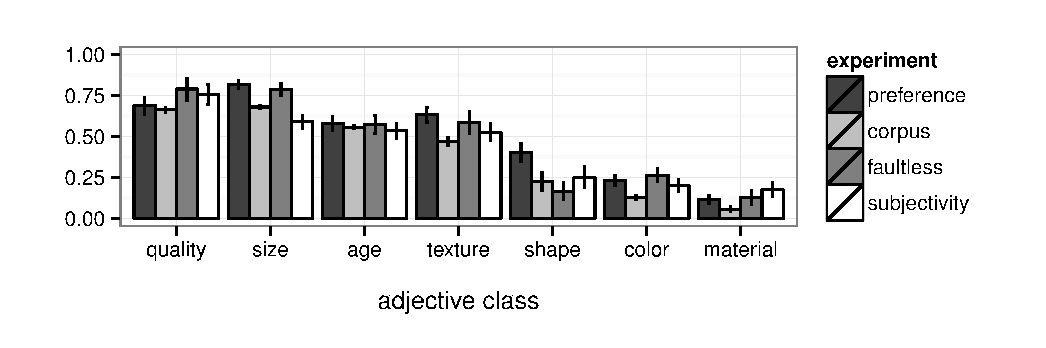
\includegraphics[width=.75\linewidth]{plots/expt_results-new.eps}}\par
	%\vspace{-10pt}
	\caption{Mean distance from noun inferred from naturalness ratings (preference), mean distance from noun calculated from corpus counts (corpus),  mean faultless disagreement ratings (faultless), and mean subjectivity ratings (subjectivity) for adjectives grouped by their semantic class. Error bars represent bootstrapped 95\% confidence intervals drawn from 10,000 samples of the data \cite{diciccioefron1996}.}\label{results}
\end{figure*}

\begin{figure}
	\centering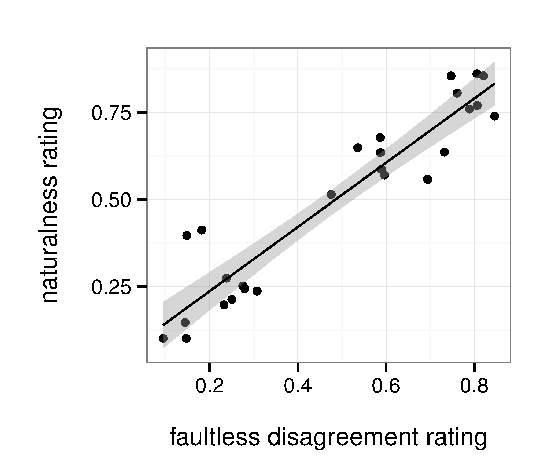
\includegraphics[width=2.8in]{plots/naturalness-faultless-new.eps}
	\caption{Mean naturalness ratings plotted against mean faultless disagreement scores for each of the 26 adjectives tested.}\label{naturalness-faultless-pred}
\end{figure}

\begin{figure}
	\centering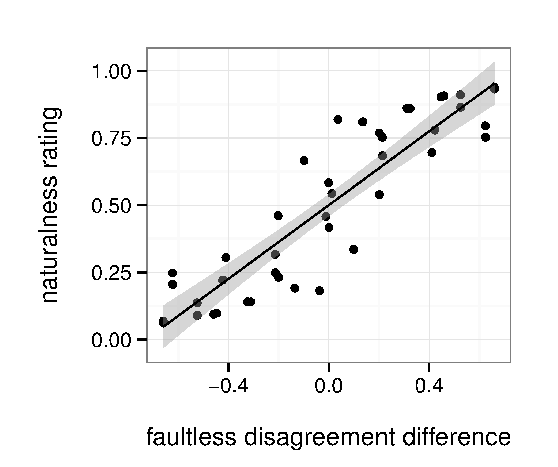
\includegraphics[width=2.8in]{plots/naturalness-faultless-configuration.eps}
	\caption{Mean configuration naturalness ratings plotted against faultless disagreement difference scores for each pair of adjective classes.}\label{naturalness-faultless}
\end{figure}


\begin{figure}[h]
	\centering
	\fbox{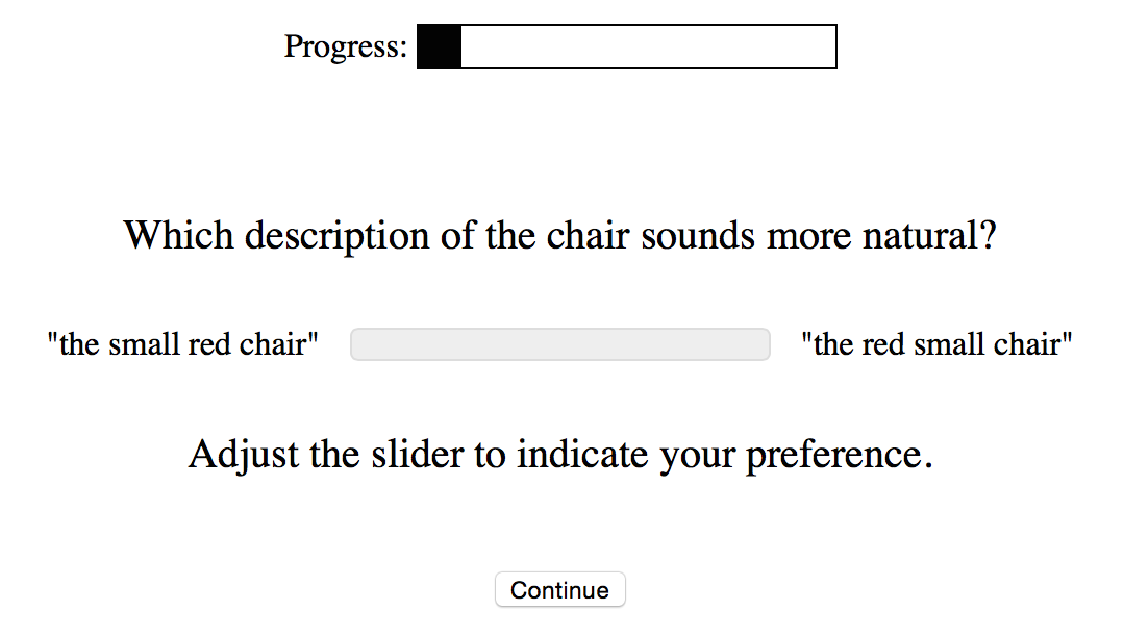
\includegraphics[width=3.3in]{images/order_trial.eps}}
	\caption{Example trial from Expt.\ 1; participants indicated the more natural of two adjective-adjective-noun descriptions on a sliding scale.}\label{order-trial}
\end{figure}

\begin{figure}[h]
	\centering
	\fbox{\includegraphics[width=3.75in]{images/faultless_trial.eps}}
	\caption{Example trial from Expt.\ 3; participants rated the potential for faultless disagreement between two speakers.}\label{faultless-trial}
\end{figure}

\begin{figure}[h]
	\centering
	\fbox{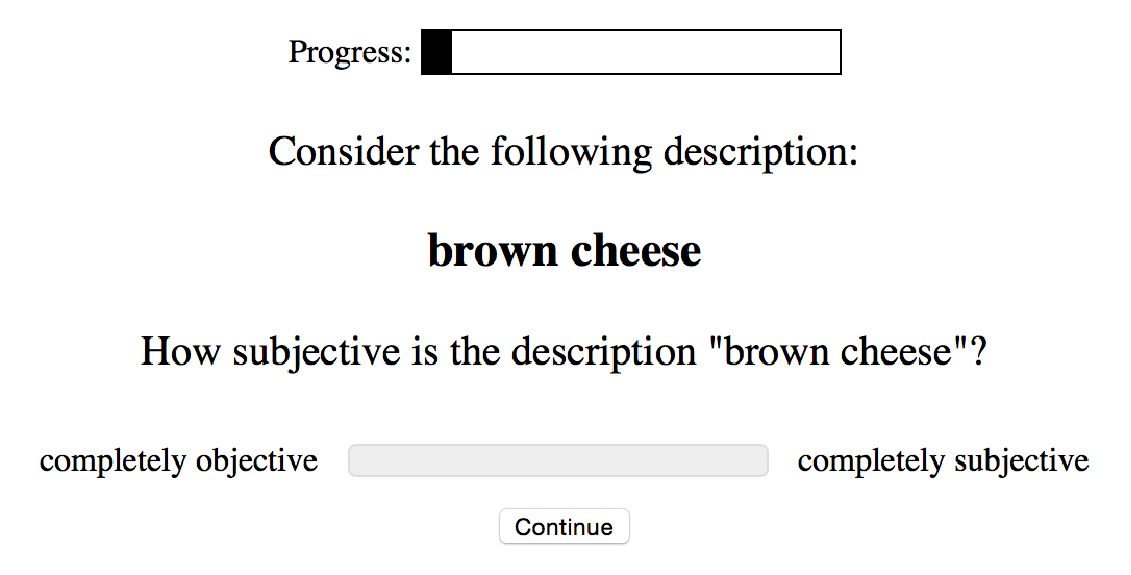
\includegraphics[width=3.3in]{images/subjectivity_trial.eps}}
	\caption{Example trial from Expt.\ 4; participants rated the subjectivity of adjective-noun object descriptions.}\label{subjectivity-trial}
\end{figure}

\begin{table}[t]
	\caption{Adjectives and their semantic classes tested in all experiments, and nouns and their classes tested in the behavioral experiments.}\label{stim-table}
	\centering{\footnotesize\begin{tabular}{@{\vrule height 10.5pt depth2pt  width0pt}llllll}
			{adjective}	&	{class}	&	{adjective}	&	{class}	&	{noun}	&	{class}	\\ \hline
			old	&	age	&	good	&	quality	&	apple	&	food	\\
			new	&	age	&	bad	&	quality	&	banana	&	food	\\
			rotten	&	age	&	round	&	shape	&	carrot	&	food	\\
			fresh	&	age	&	square	&	shape	&	cheese	&	food	\\
			red	&	color	&	big	&	size	&	tomato	&	food	\\
			yellow	&	color	&	small	&	size	&	chair	&	furniture	\\
			green	&	color	&	huge	&	size	&	couch	&	furniture	\\
			blue	&	color	&	tiny	&	size	&	fan	&	furniture	\\
			purple	&	color	&	short	&	size	&	TV	&	furniture	\\
			brown	&	color	&	long	&	size	&	desk	&	furniture	\\
			wooden	&	material	&	smooth	&	texture	\\				
			plastic	&	material	&	hard	&	texture	\\				
			metal	&	material	&	soft	&	texture	\\													
		\end{tabular}} %\label{stim-table}\caption{Adjectives and nouns used in experimental stimuli.}
\end{table}


\end{document}



